% Fakesection 序言之前

\RequirePackage[l2tabu, orthodox]{nag}
\RequirePackage{ifxetex}
\RequireXeTeX

\documentclass{ctexart}

%颜色
\usepackage{xcolor}

%长度
\usepackage{printlen}
\uselengthunit{mm}

%图形
\usepackage{pifont}
\usepackage{ean13isbn}
\usepackage{qrcode}
\usepackage{pdfpages}
\usepackage{overpic}
\usepackage{graphicx}
\graphicspath{{./src/}}
\usepackage{media9}
\usepackage{wallpaper}
\usepackage{wrapfig}

%表格
\usepackage{tabu}
\usepackage{longtable}
\usepackage{booktabs}
\usepackage{diagbox}
\usepackage{multicol}
\usepackage{multirow}
\usepackage{makecell}
\usepackage{fancybox}
\usepackage{colortbl}
\usepackage{tcolorbox}
\tcbuselibrary{skins}
\tcbuselibrary{breakable}
\tcbuselibrary{theorems}
\tcbuselibrary{listings}
\tcbuselibrary{xparse}
\tcbuselibrary{minted}% 用minted排版代码
\usepackage{fvextra}
\usepackage{csvsimple}
\usepackage{boxedminipage2e}

%公式
\usepackage{amsmath}
\usepackage{amsthm}
\usepackage{amsfonts}
\usepackage{amssymb}
\usepackage{amsbsy}
\usepackage{amsopn}
\usepackage{amstext}
\usepackage{mathrsfs}
\usepackage{bm}
\usepackage{textcomp}
\usepackage{latexsym}
\usepackage{exscale}
\usepackage{relsize}
%\usepackage{xymtex}
\usepackage{physics}
\usepackage{siunitx}
\usepackage{hologo}
\usepackage{cases}

%文字
\usepackage{csquotes}
\usepackage{microtype}

%正文
\usepackage{fancyhdr}
\usepackage{geometry}
\usepackage{lastpage}
\usepackage{indentfirst}
\usepackage{setspace}
\renewcommand\arraystretch{1.5}

%非正文
\usepackage{makeidx}
\makeindex
\usepackage{epigraph}
\usepackage{varwidth}
\usepackage{exercise}
\usepackage{tasks}

%参考文献
\usepackage{morewrites}
\renewcommand{\thefootnote}{\fnsymbol{footnote}}
\usepackage[resetlabels]{multibib}

%标题
\usepackage{caption}
\usepackage{subcaption}
\DeclareCaptionLabelFormat{andtable}%
{#1#2~\&~\tablename\thetable}
\newcounter{sub}

%其它
\usepackage{atbegshi}
\usepackage{lipsum}

\csname
endofdump
\endcsname

%代码
\usepackage{minted}
\usepackage{boxie}
\makeatletter
\xdefinecolor{tcbcol@back}{rgb}{0,0,0}
\makeatother
\usepackage{tikz}
%%MatLab命令行
\newcommand{\MatlabLogo}{%
	\begin{tikzpicture}[x=2.4ex,y=2.4ex,line width=0ex,scale=1]
		\node[draw,fill=white,text=white] at (0, 0) (a) {
				\includegraphics[width=2.4ex]{matlabLogo.ai}
			};
	\end{tikzpicture}
}
\tcbset{%
	skin=enhanced,%
	matlab/.style={%
		skin=bicolor,%
		boxrule=0.1mm,%
		%toptitle=1ex,
		sharp corners,
		breakable,%
		colbacktitle=WinGray,%
		colframe=WinGray,%
		coltitle=black,%
		fonttitle=\sffamily,%\bfseries,
		fontupper=\small\sffamily,
		fontlower=\small\sffamily,
		frame style={%
			draw=WinBlue,%
			left color=WinBlue,%
			right color=WinBlue%
		},%
		overlay unbroken = {%
			\node[inner sep=0pt,anchor=north west,yshift=-3pt,xshift=1.2pt,text=black]
			at (frame.north west){\MatlabLogo};% \fbox{\faTerminal}
			\node[inner sep=0pt,anchor=north east,yshift=-3pt,xshift=-8pt,text=black] at (frame.north
			east){\rule{0.8em}{0.6pt}\quad$\square$\quad{\Large$\times$}};
		},%
		overlay first = {%
			\node[inner sep=0pt,anchor=north west,yshift=-3pt,xshift=1.0pt,text=black]
			at (frame.north west){\MatlabLogo};%\small ~\faWindows
			\node[inner sep=0pt,anchor=north east,yshift=-3pt,xshift=-8pt,text=black] at (frame.north
			east){\rule{0.8em}{0.6pt}\quad$\square$\quad{\Large$\times$}};
		}%
	},
	matlablight/.style={
		matlab,%
		colback=white,%
		colupper=black,%
		%coltext=black%
	},
	matlabdark/.style={
		matlab,%
		colback=black,%
		colupper=white,%
		%coltext=white%
	}
}
\DeclareTCBListing{matlabdarkc}{ m m }{%
	listing engine=minted,%
	minted style=trac,%
	minted options={%
		autogobble,%
		breaklines,%
		fontsize=\wuhao,%
		baselinestretch=0.6,%
		breaksymbolleft={},%
		numbersep=3mm%
	},%
	listing and comment,%
	colbacklower=tcbcol@back!5!yellow!10!white,%
	collower=linux,%
	matlabdark,%
	title={#2},%
	comment={\small\sffamily#1},%
	minted language=bat%
}
\DeclareTCBListing{matlablightc}{ m m }{%
	listing engine=minted,%
	minted style=trac,%
	minted options={%
		autogobble,%
		breaklines,%
		fontsize=\wuhao,%
		baselinestretch=0.6,%
		breaksymbolleft={},%
		numbersep=3mm%
	},%
	listing and comment,%
	colbacklower=tcbcol@back!5!yellow!10!white,%
	collower=linux,%
	matlablight,%
	title={#2},%
	comment={\small\sffamily#1},%
	minted language=bat%
}
\DeclareTCBListing{matlabdark}{ m }{%
	listing engine=minted,%
	minted style=trac,%
	minted options={%
		autogobble,%
		breaklines,%
		fontsize=\wuhao,%
		baselinestretch=0.6,%
		breaksymbolleft={},%
		numbersep=3mm%
	},%
	listing only,%
	matlabdark,%
	title={#1},%
	minted language=bat%
}
\DeclareTCBListing{matlablight}{ m }{%
	listing engine=minted,%
	minted style=trac,%
	minted options={%
		autogobble,%
		breaklines,%
		fontsize=\wuhao,%
		baselinestretch=0.6,%
		breaksymbolleft={},%
		numbersep=3mm%
	},%
	listing only,%
	matlablight,%
	title={#1},%
	minted language=bat%
}
\newtcbinputlisting{\matlabdarkcfile}[3]{%
	listing engine=minted,%
	minted style=trac,%
	minted options={%
		autogobble,%
		breaklines,%
		fontsize=\wuhao,%
		baselinestretch=0.6,%
		breaksymbolleft={},%
		numbersep=3mm%
	},%
	listing and comment,%
	colbacklower=tcbcol@back!5!yellow!10!white,%
	collower=linux,%
	matlabdark,%
	listing file={#3},
	title={#2},%
	comment={\small\sffamily#1},%
	minted language=bat%
}% end matlabdarkcfile
% 将文件做为窗口内容的Windows终端窗口样式命令
% 第1个参数是窗口底端提示信息
% 第2个参数是窗口标题
% 第3个参数是包含窗口内容的文件全路径名称(可以是相对路径)
\newtcbinputlisting{\matlablightcfile}[3]{%
	listing engine=minted,%
	minted style=trac,%
	minted options={%
		autogobble,%
		breaklines,%
		fontsize=\wuhao,%
		baselinestretch=0.6,%
		breaksymbolleft={},%
		numbersep=3mm%
	},%
	listing and comment,%
	colbacklower=tcbcol@back!5!yellow!10!white,%
	collower=linux,%
	matlablight,%
	listing file={#3},
	title={#2},%
	comment={\small\sffamily#1},%
	minted language=bat%
}% end matlablightcfile
% 将文件做为窗口内容的Windows终端窗口样式命令
% 第1个参数是窗口标题
% 第2个参数是包含窗口内容的文件全路径名称(可以是相对路径)
\newtcbinputlisting{\matlabdarkfile}[2]{%
	listing engine=minted,%
	minted style=trac,%
	minted options={%
		autogobble,%
		breaklines,%
		fontsize=\wuhao,%
		baselinestretch=0.6,%
		breaksymbolleft={},%
		numbersep=3mm%
	},%
	listing only,%
	matlabdark,%
	listing file={#2},
	title={#1},%
	minted language=bat%
}% end matlabdarkfile
% 将文件做为窗口内容的Windows终端窗口样式命令
% 第1个参数是窗口标题
% 第2个参数是包含窗口内容的文件全路径名称(可以是相对路径)
\newtcbinputlisting{\matlablightfile}[2]{%
	listing engine=minted,%
	minted style=trac,%
	minted options={%
		autogobble,%
		breaklines,%
		fontsize=\wuhao,%
		baselinestretch=0.6,%
		breaksymbolleft={},%
		numbersep=3mm%
	},%
	listing only,%
	matlablight,%
	listing file={#2},
	title={#1},%
	minted language=bat%
}% end matlablightfile

%链接%与beamer 冲突
\usepackage
[	colorlinks = true,
linkcolor = gray,
citecolor = gray,
backref=page
]{hyperref}

%枚举%与beamer 干涉
\usepackage{enumitem}
\setlist[enumerate, 2]
{	fullwidth,
	label = \alph*.,
	font = \textup,
	itemindent=2em
}

%标题%与beamer 冲突
\usepackage{titlesec}
%\titleformat{\chapter}{\centering\Huge\bfseries}{实验\chinese{chapter}~}{0pt}{}
\titleformat{\section}{\centering\LARGE\bfseries}{\S\ifthenelse{\value{section}=0}{}{\thesection}~}{0pt}{}
%\titleformat{\subsection}{\Large}{\chinese{subsection}、~}{0pt}{}
%\titleformat{\subsubsection}{\large}{\arabic{subsubsection}.~}{0pt}{}

\begin{document}

% Fakesection 摘要

\title{\textbf{基于神经网络的二手车估价转让问题研究}}
\author{}
\date{}
\maketitle

\renewcommand{\abstractname}{\Large 摘要}
\begin{abstract}

	我国二手汽车交易量日益增加,但二手车市场存在严重的信息不对称,缺乏可信的价格评估体系。设计评估二手汽车价格的模型、使用模型对二手汽车交易行为进行分析是亟待解决的问题。

	针对问题一,我们建立了”二手车价格评价模型“。首先,我们确定了影响二手车交易价格的关键因素。随后,我们运用神经网络算法得到二手汽车价格与关键因素之间的定量函数关系,并整体误差下降趋势、系统梯度、计算值与实际值的相关关系等神经网络性能进行评估。

	针对问题二,我们基于问题一的模型,固定除行驶里程之外的关键因素,以行驶里程为自变量,计算得到了A级车、B级车、C级车、SUV车二手价格随行驶里程的变化曲线。

	针对问题三,首先,我们基于问题一的模型,采用控制变量法,固定除行驶里程和使用时间之外的关键因素,以行驶里程和使用时间为自变量,分析此双变量系统,计算得到了二手汽车价格随行驶里程的变化曲线。随后,我们分析上述曲线,寻找曲线拐点、峰值、突变等特征,计算得出一手车主最佳卖出年份或最佳卖出里程数。

	综上,我们解决了题目所给问题,并将在未来完善模型,以扩大适用范围。
\end{abstract}

\textbf{关键词:二手车价格,神经网络,控制变量,行驶里程}

\newpage

% Fakesection 目录

\pagenumbering{roman}

\tableofcontents

\newpage

\listoffigures

\newpage

\listoftables

\newpage

\setcounter{section}{-1}

\pagenumbering{arabic}

\section{引言}%
\label{sec:引言}

\subsection{问题背景}%
\label{sub:问题背景}
十九大以来,交通强国建设成为政府重点关注的国家工程之一,这有效地带动了我国汽车产业迅猛发展。

在这一背景下,民众生活水平的提高,使得汽车的需求量、生产量、交易量日益增长,汽车更新换代加快,新车交易渐渐趋向饱和,许多人开始倾向于购买二手汽车。国外的二手车交易体系相当成熟,拥有完善的法规体系,多样的交易方式。而我国二手车市场存在严重的信息不对称,也没有相对可信的价格评估体系。

设计评估二手汽车价格的模型、使用模型对二手汽车交易行为进行分析是亟待解决的问题。

\subsection{问题重述}%
\label{sub:问题重述}
人们会根据各种因素来抉择:乘坐高铁还是火车。
\begin{enumerate}
	\item 考虑地区、品牌、新车价格、里程、交通事故维修价值、汽车状况,提出计算二手汽车买卖价格的模型。
	\item 在A级车(紧凑型轿车),B级车(中型轿车车),C级车(中大轿车) 和SUV型车中各选一款车,利用所提模型计算价格随行驶里程的变化曲线。
	\item 考虑随着使用时间的延长,汽车的事故率会呈现指数形式增长,建立模型计算一手车主最佳卖出年份或最佳卖出里程数。

\end{enumerate}
\newpage

\section{问题分析}%
\label{sec:问题分析}

\subsection{问题一}
首先,我们确定了影响二手车交易价格的关键因素。随后,我们建立了“二手汽车价格计算模型”,运用神经网络算法得到二手汽车价格与关键因素之间的定量函数关系。 \cite{周志华-机器学习}

\subsection{问题二}
我们基于问题一的模型,固定除行驶里程之外的关键因素,以行驶里程为自变量,计算得到了A级车、B级车、C级车、SUV车二手价格随行驶里程的变化曲线。 %\cite{u014303046}

\subsection{问题三}
首先,我们基于问题一的模型,采用控制变量法,固定除行驶里程和使用时间之外的关键因素,以行驶里程和使用时间为自变量,分析此双变量系统,计算得到了二手汽车价格随行驶里程的变化曲线。随后,我们分析上述曲线,寻找曲线拐点、峰值、突变等特征,计算得出一手车主最佳卖出年份或最佳卖出里程数。

\subsection{假设}%
\label{sub:假设}

\begin{enumerate}
	\item 通过网络获取的二手车交易数据均真实可靠。
	\item 在模型运用阶段,模型应用的地区不发生金融危机、通货膨胀、战争战乱等影响二手车交易价格的极端因素。
	\item 所提二手车的生产制造及使用均合法合规。
	\item 人们对于二手车的喜爱偏好短期内不会发生改变。
\end{enumerate}





\newpage

\section{问题一}%
\label{sec:问题一}
\subsection{筛选影响二手车价格的主要因素}
首先,我们确定了影响二手车交易价格的关键因素,即初始价格、购买年份、里程、是否有补贴,并通过在网络上查找到了相关交易数据。 %\cite{wuaini-1314}
\subsection{神经网络算法原理设计}
\subsubsection{神经元}
神经元模型是模拟生物神经元结构而被设计出来的。神经元大致可以分为树突、突触、细胞体和轴突。树突为神经元的输入通道,其功能是将其它神经元的动作电位传递至细胞体。其它神经元的动作电位借由位于树突分支上的多个突触传递至树突上。神经细胞可以视为有两种状态的机器,激活时为“是”,不激活时为“否”。神经细胞的状态取决于从其他神经细胞接收到的信号量,以及突触的性质(抑制或加强)。当信号量超过某个阈值时,细胞体就会被激活,产生电脉冲。电脉冲沿着轴突并通过突触传递到其它神经元。\textcolor{red}{[1]}


同理,我们的神经元模型就是为了模拟上述过程,典型的神经元模型如下:\textcolor{red}{[2]}
\renewcommand\figurename{图}
\begin{figure}[H]
	\centering
	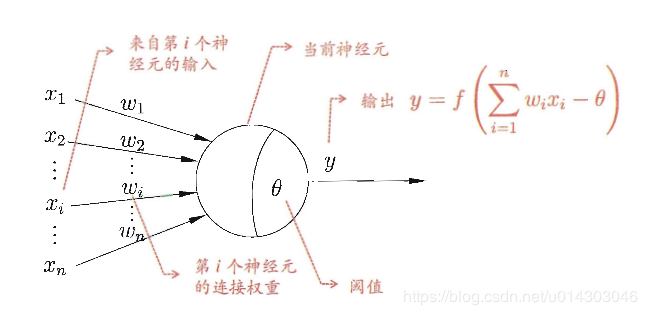
\includegraphics[width=13cm]{shenjing.png}
	\caption{神经元模型} \label{all}
\end{figure}

\subsubsection{神经网络结构}
本文所用的神经网络为四层(含输入层与输出层)[4,10,10,1]神经元数量的结构体,如下图所示:
\renewcommand\figurename{图}
\begin{figure}[H]
	\centering
	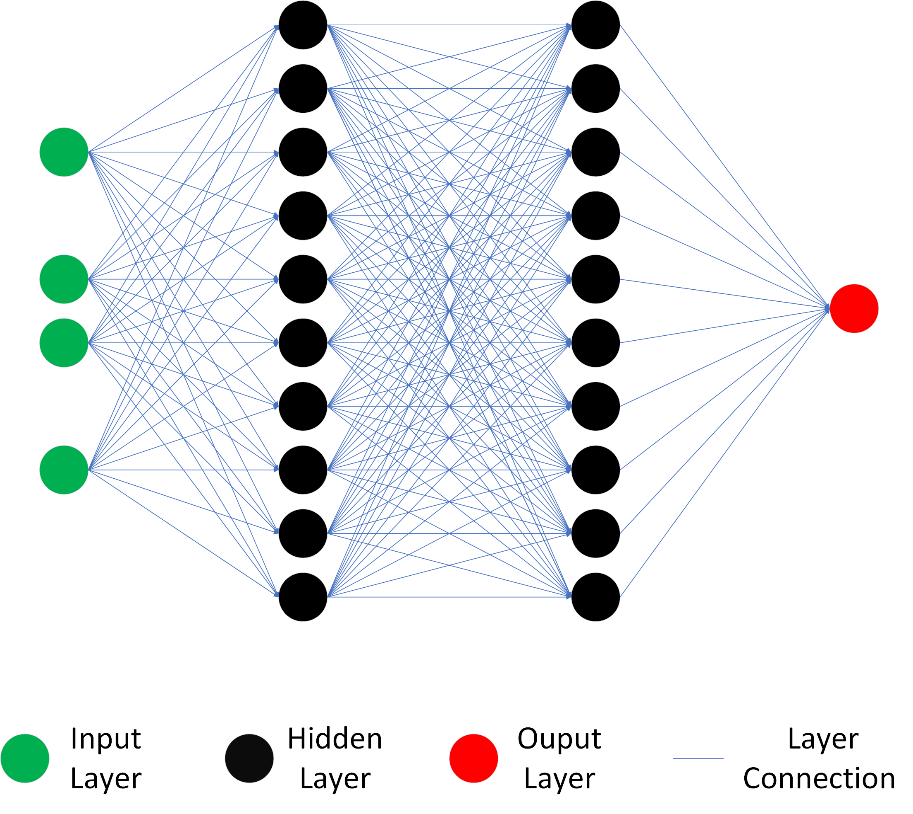
\includegraphics[width=8cm]{jiegou.png}
	\caption{神经网络结构} \label{all}
\end{figure}

\subsubsection{反向传播}
本文所搭建的神经网络采用LM迭代法来进行反向传播。LM迭代法是介于牛顿法与梯度下降法之间的一种算法。
\renewcommand\figurename{图}
\begin{figure}[H]
	\centering
	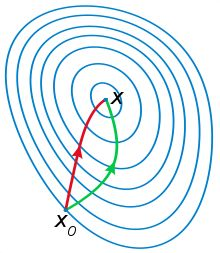
\includegraphics[width=5cm]{fanxiang.png}
	\caption{LM迭代法(红为牛顿,绿为梯度下降)} \label{all}
\end{figure}

梯度下降主要是从一阶目标函数的一阶导推导而来的,形象点说,就是每次朝着当前梯度最大的方向收敛;二牛顿法是二阶收敛,每次考虑收敛方向的时候,还会考虑下一次的收敛的方向是否是最大。具体的来讲,梯度下降法由于下降速度过快,容易陷入到局部最优解,与之相对的,牛顿法虽然下降速度慢,但是对于最优解的寻取效果好。

高斯-牛顿和LM法则主要是针对非线性最小二乘问题提出的解决方案。由于牛顿法需要求解二阶导,也就是hessian matrix,运算量大,不利于实现,,所以通常在牛顿法的基础上用去掉二阶项,用一阶项来近似二阶导,从而保证了计算效率。LM方法,则是由于高斯-牛顿方法在计算时需要保证矩阵的正定性,于是引入了一个约束,从而保证计算方法更具普适性。\textcolor{red}{[3]}

\subsection{使用神经网络算法设计计算二手汽车价格的模型}
本文将二手车的初始价格,购入年份,行驶距离,是否有补贴为输入指标,采用tansig传递函数,二手车的买卖价格为输出指标。由于本文所基于的数据量较小,故我们对每一辆车进行单独分析,来证明算法的可行性。若数据量形成一定规模,可将汽车的品牌型号单独列为指标,采用softmax传递函数,输入至网络之中。 %\cite{卓金武-MATLAB在数学建模中的应用}

网络收敛效果如下:
\renewcommand\figurename{图}
\begin{figure}[H]
	\centering
	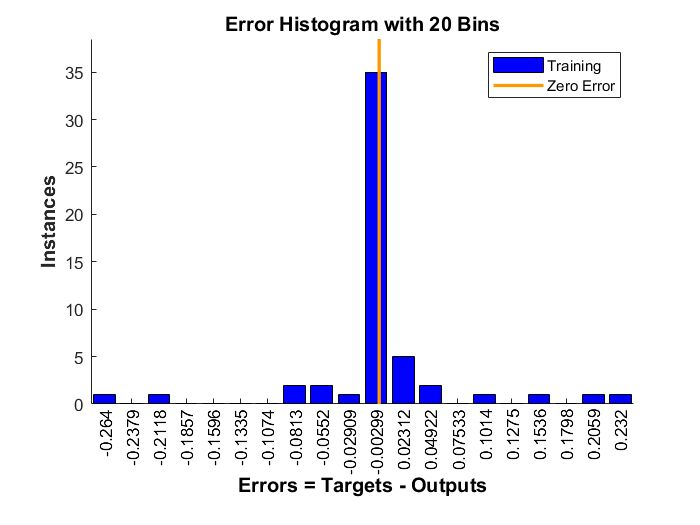
\includegraphics[width=10cm]{a.jpg}
	\caption{所有数据通过神经网络计算出的值与实际值之间的误差} \label{all}
\end{figure}

\renewcommand\figurename{图}
\begin{figure}[H]
	\centering
	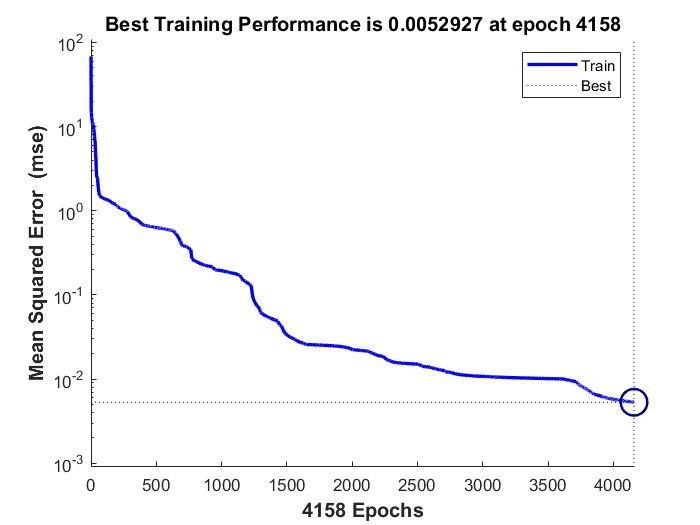
\includegraphics[width=10cm]{b.jpg}
	\caption{随着神经网络反向传播次数的增加整体误差的下降趋势} \label{all}
\end{figure}

\renewcommand\figurename{图}
\begin{figure}[H]
	\centering
	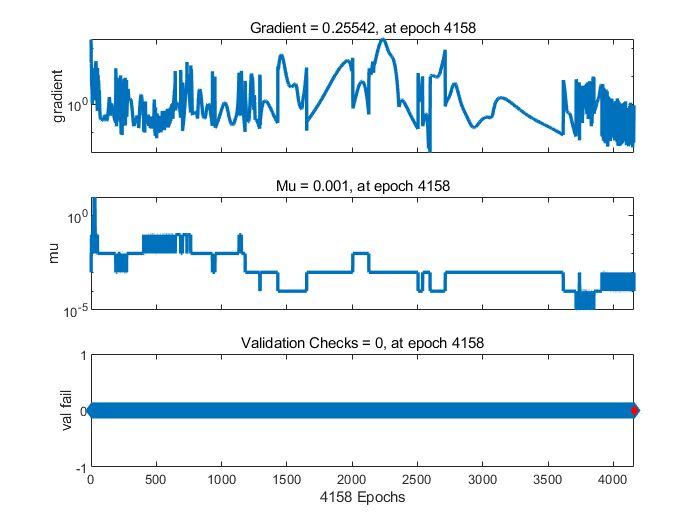
\includegraphics[width=10cm]{c.jpg}
	\caption{下降过程中系统梯度、梯度修正系数、下降失败的次数} \label{all}
\end{figure}

\renewcommand\figurename{图}
\begin{figure}[H]
	\centering
	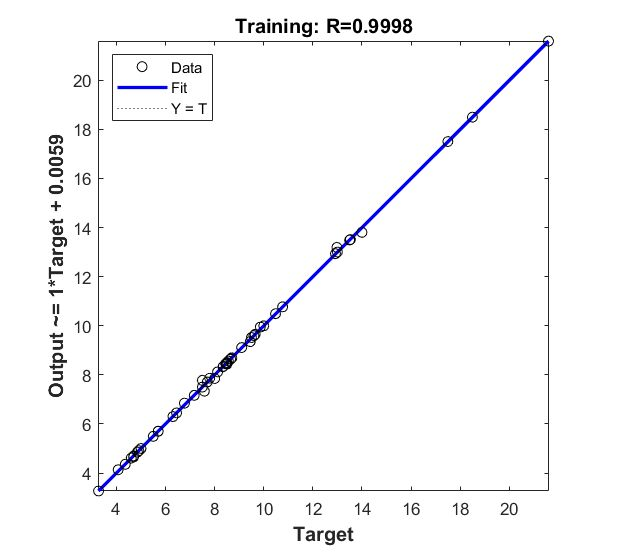
\includegraphics[width=10cm]{d.jpg}
	\caption{最终结果神经网络计算值与实际值的相关关系} \label{all}
\end{figure}

最终得到的二手车价格计算公式如下:
\begin{equation}
	Y=W_3 \dot SIGTAN(W_2 \dot sigtan(W_1 \dot X+B_1)+B_2)+B_3
\end{equation}
其中:

$W_1$是一个10行4列的矩阵,它的元素从左到右从上到下依次是: \cite{姜启源-数学模型}

20.3651965424134,	-14.5402678321673,	9.78464598058885,	-3.65719645796286,
-3.93075206987240,	-52.0726087129351,	89.0943491266983,	-11.6332435795027,
22.0578792577284,	1.94251755262784,	10.4553188361080,	7.16433155513226,
9.58824739294488,	8.58045555893562,	17.8120880160124,	-12.0161740684939,
-17.4780968879099,	-4.12398815983475,	2.33906273791870,	-2.63497599632593,
-13.6926444761707,	-22.8195018519429,	-33.8684246837968,	6.98946479567157,
-2.70727982566091,	-17.9194911385383,	8.63662439174050,	8.06765537470396,
40.4640160468195,	-2.61058578619659,	2.53131880258979,	-7.83126740502195,
3.04428475621333,	-5.24067200327106,	-8.90712468940171,	-7.67222413128319,
-3.72863511589714,	-8.34829801307679,	11.0619670504835,	0.0294310636711716。

$W_2$是一个10行10列的矩阵,它的元素从左到右从上到下依次是:

30.1249853434453,	-1.94187566195855,	-4.08986945984398,	-10.1867069269422,	-5.37128507110402,	-14.0487462852381,	5.21485311522263,	-23.1311728292925,	1.25242560313738,	-4.24219619857368,
25.7227541391500,	-0.0174665174344685,	0.409837299919951,	39.7268169518885,	24.7710396844911,	-4.68446426673656,	-2.09100432478755,	44.0323959865757,	-7.21711768971998,	-8.65654239365764,
-0.369019364980948,	-7.32686164656248,	2.56622862650220,	10.2971928135057,	-2.94573157767923,	1.04846286765719,	5.25242460077063,	-45.6085752854114,	7.14117027973796,	-8.82410803167194,
18.2784507751144,	3.11950561201561,	-2.73884356937015,	13.0413025040044,	1.25005943675594,	8.95745038901308,	-12.3128101854690,	-7.68368670651581,	-14.6890972586014,	0.703057597784747,
28.2021982884502,	-3.41770785594564,	11.4052026652238,	20.1406221614397,	9.72161273782509,	-1.33907927258118,	-3.27072476025516,	-43.0550935779320,	21.9579449568575,	-2.33983268706680,
-2.47814991865985,	0.740235388812245,	-2.06609239561799,	0.890893869320478,	2.21374460235646,	-1.39423387156234,	4.88155595442679,	0.238324923120211,	-0.519983772705202,	4.83458241225971,
4.16854181135854,	4.36641689429232,	19.6812100393535,	-2.75047226634913,	6.32508120139995,	-7.65034109120620,	-10.9826098231678,	2.74992195010882,	5.06031921594004,	10.9083360806471,
-3.12478303864535,	-1.98836930835631,	-7.25765202618144,	6.13250230157260,	-14.0950516444746,	-13.0843733214942,	-0.434289253789550,	-34.4181891440557,	37.9666830146348,	7.19699016112823,
0.597995713533756,	0.637034249913943,	4.56662280740570,	1.06618573065219,	27.0475880268654,	-2.19953772656098,	-2.35094519691665,	4.73709740948661,	-7.81675214406592,	-5.51681972662072,
-3.09190667169788,	-4.89640528114553,	1.38394311545609,	7.47801244226033,	7.47732358827146,	9.60968613218010,	-0.839108272730330,	2.79295787284196,	-2.83920914458334,	-1.51810783469511。

$W_3$是一个1行10列的矩阵,它的元素从左到右从上到下依次是:
37.6691045545207,	-24.1456589546345,	-35.2662733032427,	9.03253192881971,	-26.2972428939178,	-5.82538110010033,	22.9959728588659,	34.9630084803163,	-11.9565963303093,	50.4409618432971。

$B_1$是一个10行1列的矩阵,它的元素从左到右从上到下依次是:
-12.6758159714683,
-0.813463688049872,
-3.32890715751604,
3.29103314384604,
-6.02583123228726,
-28.7415219129422,
-4.07645127076633,
-9.94893334695816,
-16.6596865644290,
-1.25950398810596。

$B_2$是一个10行1列的矩阵,它的元素从左到右从上到下依次是:
18.2344912155943,
-6.15193187253280,
3.26470993235194,
-9.56971966901664,
-9.65559877955475,
4.33987952608641,
-2.16491492543118,
7.63280543876187,
4.82696632178034,
-8.19554615346707。

$B3=-3.8611$。


\newpage
\section{问题二}%
\label{sec:问题二}

根据本文第一问所建立的模型,我们对A级车(紧凑型轿车),B级车(中型轿车),C级车(中大轿车)和SUV型车中的某一款车计算随行驶里程的变化曲线。
\subsection{紧凑型汽车}
本文紧凑型汽车选取别克英朗系列。

物理学中对于多因素(多变量)的问题,常常采用控制因素(变量)的方法,即把多因素的问题变成多个单因素的问题。每一次只改变其中的某一个因素,而控制其余几个因素不变,从而研究被改变的这个因素对事物影响,分别加以研究,最后再综合解决。故本文也采用采用控制变量法,首先假设汽车的使用寿命为1年,初始价格为12万元,对汽车的行驶距离进行变更,来观察汽车价格的变化,如图所示:
\renewcommand\figurename{图}
\begin{figure}[H]
	\centering
	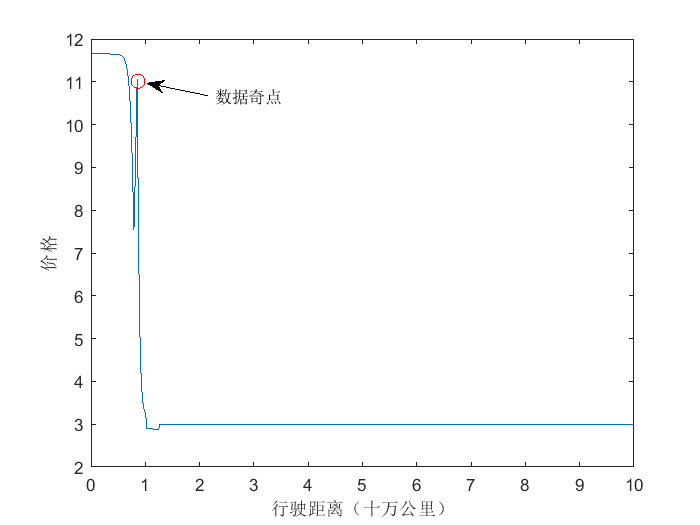
\includegraphics[width=10cm]{one.png}
	\caption{价格随行驶距离的变化} \label{all}
\end{figure}

可以发现,在行驶距离超过10万公里时,发生了一个较大的数据滑坡,这意味着如果车辆该品牌的车辆在新购买一年内行驶超过10万公里时,可能车辆的事故率或者车辆的质量会发生一个较大层面的提升,从而导致了车辆的急速贬值。

在图中出现了一个数据异常上升,第一点可能由于当行驶距离处于10万公里左右时,车辆的具体价值不容易界定;第二点可能由于训练集的数据规模较小,在没有训练充足,由于少数异常点的存在,学习了错误的定价规律。分析数据集,出现第一种情况的可能性较大。

\subsection{中型轿车}
本文中型轿车选取了本田的INSPIRE系列车型。同样利用控制变量法,与之前类似,假设汽车的使用寿命为1年,初始价格为12万元,对汽车的行驶距离进行变更,来观察汽车寿命的变化。最终的结果如图所示。
\renewcommand\figurename{图}
\begin{figure}[H]
	\centering
	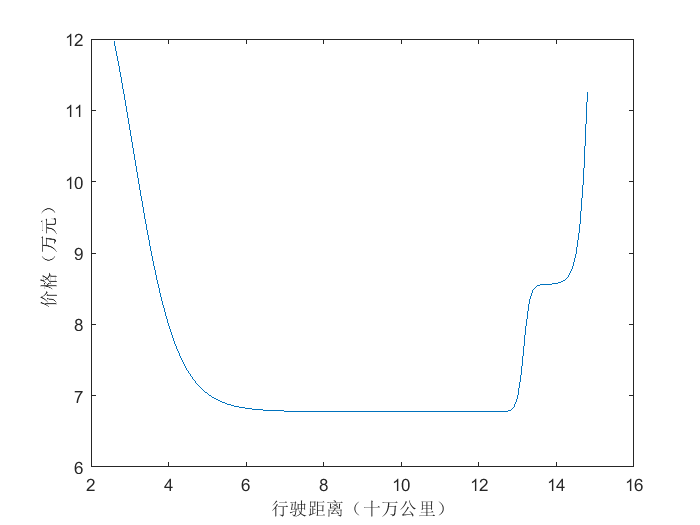
\includegraphics[width=10cm]{two.png}
	\caption{价格随行驶距离的变化} \label{all}
\end{figure}

可以看出,汽车的价格下降相对于别克的紧凑型汽车相对坡度较小,在第60万公里时价值衰减至最低点,值得注意的是,此时的价格最低点为7万元左右,其保值性要远远好于别克系列。

这个出现了数据的异常回升,在第12万公里时价格反向升高,这极有可能时上一章节所述的第二点原因:由于训练集的数据规模较小,在没有训练充足,由于少数异常点的存在,学习了错误的定价规律。

\subsection{SUV}

本文SUV型车选取了马自达的CX-8系列车型。同样利用控制变量法,与之前类似,假设汽车的使用寿命为1年,初始价格为12万元,对汽车的行驶距离进行变更,来观察汽车寿命的变化。最终的结果如图所示。
\renewcommand\figurename{图}
\begin{figure}[H]
	\centering
	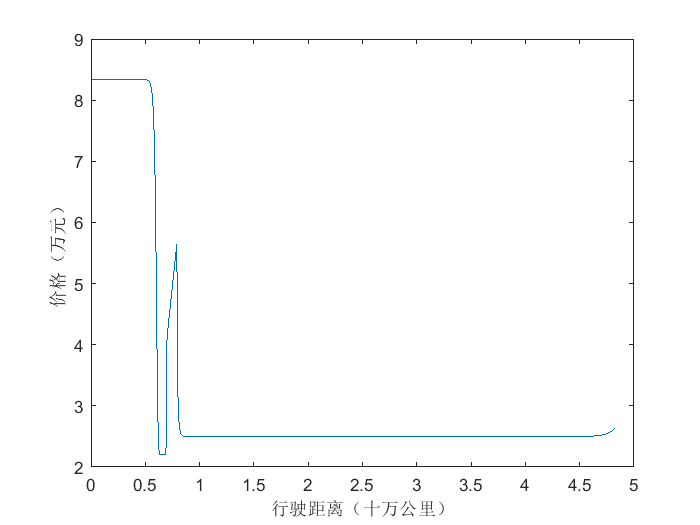
\includegraphics[width=10cm]{three.png}
	\caption{价格随行驶距离的变化} \label{all}
\end{figure}

首先可以发现,马自达系列的车型出现了入手贬值的特点,即对于12万的车辆直接贬值至8.5万元左右。第二是在0.5万公里的时候就发生了剧烈贬值,这远快于别克系列车辆与本田系列车辆,但是这一现象与SUV运动型多用途汽车的使用定位相吻合,其可能行驶条件等相对于其他用途车辆较为恶劣,这也导致了车辆的损伤速度和事故率可能有所提高。且出现了与前文别克车相类似的定价模糊现象。这一现象同样可以用之前的理论解释:贬值的梯度过大导致具体发生贬值的边界难以确定。


\newpage
\section{问题三}%
\label{sec:问题三}
与第二相类似,本问采用控制变量法,对双变量系统进行分析。在第二问的基础上,受限于收集的数据集规模,首先选取本田全系列车进行分析。
\renewcommand\figurename{图}
\begin{figure}[H]
	\centering
	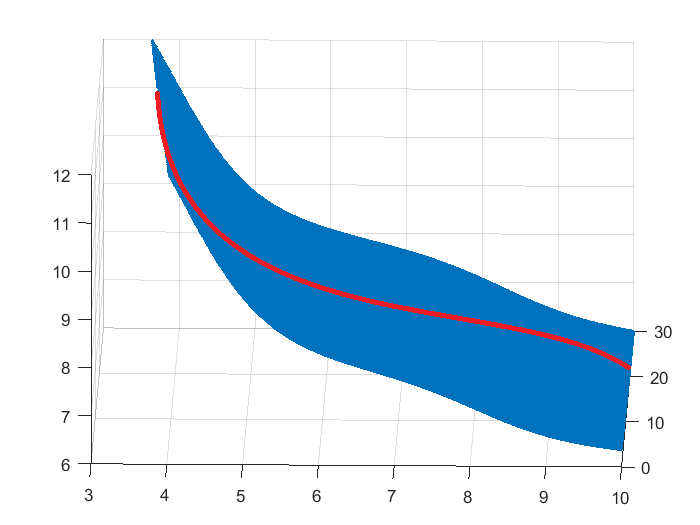
\includegraphics[width=10cm]{for.png}
	\caption{图像中3-10范围对应的坐标轴为行驶距离(十万公里),0-30范围对应的坐标轴为时间(0.2年),Z方向坐标为价格。} \label{all}
\end{figure}

与之前的结论类似,本田系列的车的保值性非常良好,从随机某一点开始做最快梯度下降曲线(如红线所示),在曲线也未出现加大的起伏。故对于本田系列的车,在任何时间或行驶里程中进行二手车买卖无明显区别。

进一步分析别克车辆与马自达车辆,如图所示:
\renewcommand\figurename{图}
\begin{figure}[H]
	\centering
	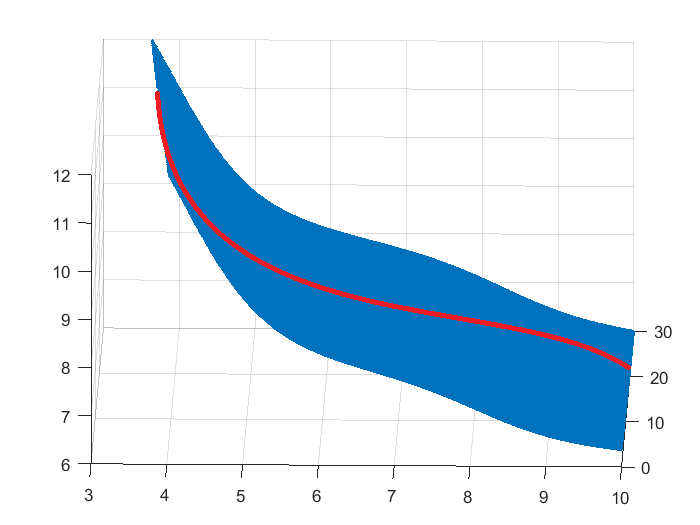
\includegraphics[width=10cm]{for.png}
	\caption{别克} \label{all}
\end{figure}

\renewcommand\figurename{图}
\begin{figure}[H]
	\centering
	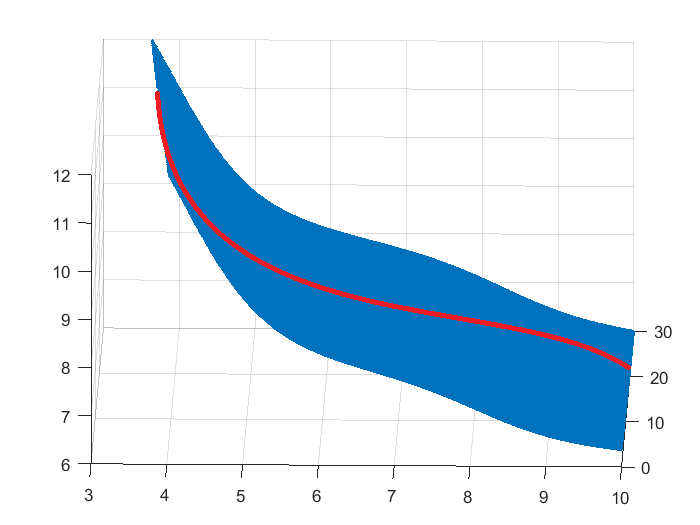
\includegraphics[width=10cm]{for.png}
	\caption{马自达} \label{all}
\end{figure}

图像中3-10范围对应的坐标轴为行驶距离(十万公里),0-30范围对应的坐标轴为时间(0.2年),Z方向坐标为价格。

对于别克系列车辆与马自达系列车辆,其都存在的明显的断崖式下降现象,最佳的卖出和使用应该建立在不穿越断崖线(如图中所示)。



\newpage

\section{模型的评价与改进}%
\label{sec:模型的评价与改进}

\subsection{优点}%
\label{sub:优点}
\begin{enumerate}
	\item 通过对数据的分析确定二手车价格评价模型,避免了主观因素对模型设计带来的偏差。
	\item  运用了神经网络算法,充分利用了交易数据,得到了较为客观的二手车价格评价模型。
\end{enumerate}

\subsection{缺点}%
\label{sub:缺点}
\begin{enumerate}
	\item 对影响二手车价格的因素的选取没有采用精确的模型。 \cite{司守奎,孙玺菁-数学建模算法与应用}
	\item 受交易隐私性的限制,网络上可以获取的二手车交易数据受限,模型设计存在误差。
\end{enumerate}

\newpage

% Fakesection 参考文献

\section{参考文献}%
% Fakesection 参考文献

\bibliographystyle{IEEEtran}
\bibliography{src/main}

\newpage

% Fakesection 附录

\renewcommand{\thesection}{\Alph{section}~}

\appendix

\section{代码}%
\label{sec:代码}

\subsection{全局清理}

\langCVfile[Matlab][code:cleanGlobal.m][Matlab]{cleanGlobal.m}{src/cleanGlobal.m}
\subsection{数据切割}

\langCVfile[Matlab][code:dataSplit.m][Matlab]{dataSplit.m}{src/dataSplit.m}
\subsection{具体分析}

\langCVfile[Matlab][code:analysize.m][Matlab]{analysize.m}{src/analysize.m}
% Fakesection 索引

\printindex

\end{document}

